\documentclass{article}
\usepackage[a4paper,margin=1.5cm]{geometry}
\usepackage[utf8]{inputenc}

\title{Dynamic labeling}
\author{Elad Noor, Evgeny Onishchenko}

\usepackage{natbib}
\usepackage{graphicx}
\usepackage{amsthm}
\usepackage{amsmath}
\usepackage{amssymb}
\usepackage{mathtools}
\usepackage{hyperref}
\usepackage{pgfplots}

\usepgfplotslibrary{colorbrewer}
\pgfplotsset{cycle list/Set1-8}
\pgfplotsset{compat=1.15}

\newtheorem{theorem}{Theorem}[section]
\newtheorem{corollary}{Corollary}[theorem]
\newtheorem{lemma}[theorem]{Lemma}
\newcommand{\finit}{\vec{f}^\circ}

\begin{document}

\maketitle

\section{General solution for dynamic labeling experiments}
Imagine a general metabolic network, which can be described as a standard graph, i.e. all reactions are one-to-one (typically, metabolic networks for medium size or larger will not qualify here, and it would be necessary to use an atom-mapping network for them).

We assume the system is at metabolic steady state, i.e. therefore all fluxes and pool sizes are constant and given by $v_{i \rightarrow j}$ (the flux from $S_i$ to $S_j$) and $s_i$ (the pool size of $S_i$). We define $v_{i \rightarrow i} = 0$. The labeled fractions are not at steady-state and we aim to describe their time evolution, denoted $f_i(t) \equiv s_i^1(t) / (s_i^0(t) + s_i^1(t)) = s_i^1(t) / s_i$. Note that $s_i$ is not a function of time, since it is assumed to be at steady-state. Then:
\begin{eqnarray}
    \frac{d s_i^0}{dt} &=& \sum_j f_j~v_{j \rightarrow i} ~~-~~ \sum_j f_i~v_{i \rightarrow j} = \\
    &=& \sum_j f_j~v_{j \rightarrow i} ~~-~~ f_i \sum_j v_{i \rightarrow j}
\end{eqnarray}
We can divide both sides by $s_i$ to get:
\begin{eqnarray}
    \frac{d f_i}{dt} = \sum_j \frac{v_{j \rightarrow i}}{s_i} \cdot f_j ~~-~~ \sum_j \frac{v_{i \rightarrow j}}{s_i} \cdot f_i
\end{eqnarray}

Now, if we rewrite this system of equations in matrix notation, we see that $\vec{f}(t)$ (the vector of all labeled fractions) is described by a homogenous system of first order differential equations:
\begin{eqnarray}\label{eq:homogenous}
    \frac{d\vec{f}}{d t} = \mathbf{M} \cdot \vec{f}
\end{eqnarray}
where $\mathbf{M}$ is a square matrix, defined by:
\begin{eqnarray}
    M_{i \neq j} &=& \frac{v_{j \rightarrow i}}{s_i}\\
    M_{ii} &=& -\frac{1}{s_i}\sum_{j} v_{i \rightarrow j}
\end{eqnarray}
or in other words, if $\mathbf{V}$ is the flux matrix (where $V_{ij} = v_{i \rightarrow j}$) then:
\begin{eqnarray}
    \mathbf{M} = \text{diag}(\vec{s})^{-1} \cdot \left( \mathbf{V}^\top - \text{diag}(\mathbf{V}^\top~\vec{1}_n) \right)
\end{eqnarray}

\subsection{Homogeneous linear system of ODEs}
We just showed that the steady-state dynamic labeling problem is a homogenous linear system of ODEs:
\begin{eqnarray}
    \frac{d\vec{f}}{d t} &=& \mathbf{M} ~ \vec{f}(t) \\
    \vec{f}(0) &=& \finit
\end{eqnarray}
which has the general solution:
\begin{eqnarray}
    \vec{f}(t) = e^{\mathbf{M} t}~\finit =  \mathbf{P}~e^{\mathbf{J}\,t}~\mathbf{P}^{-1}~\finit
\end{eqnarray}
where $\mathbf{J}$ is the Jordan normal form of $\mathbf{M}$, i.e. $\mathbf{P}~\mathbf{J}~\mathbf{P}^{-1} = \mathbf{M}$. When $\mathbf{J}$ is a diagonal matrix $\text{diag}\left(\vec{\lambda} \right)$, we can change the multiplication order, so that the formula takes on a simpler form $\vec{f}(t) = \mathbf{A} e^{\vec{\lambda} t}$:
\begin{eqnarray}\label{eq:homogenous_solution}
    \vec{f}(t) = \mathbf{P}~ \text{diag}\left(e^{\vec{\lambda} t}\right) ~\mathbf{P}^{-1}~\finit = \mathbf{P}~\text{diag}\left( \mathbf{P}^{-1} ~\finit\right)~ e^{\vec{\lambda} t}\,.
\end{eqnarray}

\subsection{Example: linear pathway with only irreversible steps}
Imaging a cascade of reactions which is at steady state, but the fluxes are not necessarily equal (e.g. there could be irreversible branching fluxes that are not considered as part of the system):
\begin{equation}
    \xrightarrow{v_1} S_0 
    \xrightarrow{v_1} S_1 
    \xrightarrow{v_2} S_2
    \xrightarrow{v_3} \ldots 
    \xrightarrow{v_n} S_n
    \rightarrow \varnothing
\end{equation}
At time $t = 0$, the first pool ($S_0$) is replaced with a fully labeled one, while all downstream pools start completely unlabeled. In addition, we define $\tau_i \equiv \frac{s_i}{v_i}$, then the $\mathbf{M}$ matrix will be:
\begin{eqnarray}
\mathbf{M} =
  \begin{bmatrix}
    0 & 0 & 0 & 0 & \ldots & 0 & 0\\
    1/\tau_1 & -1/\tau_1 & 0 & 0 & \ldots & 0 & 0\\
    0 & 1/\tau_2 & -1/\tau_2 & 0 & \ldots & 0 & 0\\
    0 & 0 & 1/\tau_3 & -1/\tau_3 & \ldots & 0 & 0\\
    & & & \vdots & & &\\
    0 & 0 & 0 & 0 & \ldots & 1/\tau_n & -1/\tau_n \\
  \end{bmatrix}
  ~~~~
  \finit = 
  \begin{bmatrix}
  1 \\ 0 \\ 0 \\ 0 \\ \vdots \\ 0
  \end{bmatrix}
\end{eqnarray}

Note that the first row in $\mathbf{M}$ is all zeros since it represents the coefficients of the time derivative of $d f_0/dt$ which is equal to $0$. To describe the solution for this ODE system, we first define $\forall i \neq j:~g_{ij} \equiv (1 - \tau_i/\tau_j)^{-1}$, and $\forall i:~g_{ii} \equiv 1$. The Jordan normal form of $\mathbf{M}$ can be expressed by (we used \href{https://www.sympy.org/}{Sympy} to find it):
\begin{eqnarray}
\mathbf{P} =
  \begin{bmatrix}
    1 & 0 & 0 & \ldots & 0 \\
    1 & (g_{21}\cdot g_{31} \cdots g_{n1})^{-1} & 0 & \ldots & 0 \\
    1 & (g_{31}\cdot g_{41} \cdots g_{n1})^{-1} & (g_{32}\cdot g_{42} \cdots g_{n2})^{-1} & \ldots & 0 \\
    1 & (g_{41}\cdot g_{51} \cdots g_{n1})^{-1} & (g_{42}\cdot g_{52} \cdots g_{n2})^{-1} & \ldots & 0 \\
    1 & (g_{51}\cdot g_{61} \cdots g_{n1})^{-1} & (g_{52}\cdot g_{62} \cdots g_{n2})^{-1} & \ldots & 0 \\
     & \vdots & & & & \\
    1 & 1 & 1 & \ldots & 1
\end{bmatrix}
~~~~
\mathbf{J} =
  \begin{bmatrix}
    0 & 0 & 0 & \ldots & 0 \\
    0 & -\frac{1}{\tau_1} & 0 & \ldots & 0 \\
    0 & 0 & -\frac{1}{\tau_2} & \ldots & 0 \\
    0 & 0 & 0 & \ldots & 0 \\
     & \vdots & & & & \\
    0 & 0 & 0 & \ldots & -\frac{1}{\tau_n}
\end{bmatrix}
\end{eqnarray}


Then, we used \href{https://www.sympy.org/}{Sympy} again to find a general expression for $\mathbf{P}^{-1} ~\finit$:
\begin{eqnarray}
    \mathbf{P}^{-1} ~\finit = 
    \begin{bmatrix}
        1 \\
        -\prod_1^n g_{i1} \\
        -\prod_1^n g_{i2} \\
        -\prod_1^n g_{i3} \\
        -\prod_1^n g_{i4} \\
        \vdots \\
        -\prod_1^n g_{in}
    \end{bmatrix}
\end{eqnarray}
and if we multiply $\mathbf{P}$ by $\text{diag}\left(\mathbf{P}^{-1}\right)$, we get:
\begin{eqnarray}
    f(t) =
    \mathbf{P}~\text{diag}\left(\mathbf{P}^{-1} ~\finit\right)~e^{\vec{\lambda}t} =
    \begin{bmatrix}
        1 & 0 & 0 & 0 & \ldots & 0 \\ \\
        1 & -\prod_1^1 g_{i1} & 0 & 0 & \ldots & 0 \\ \\
        1 & -\prod_1^2 g_{i1} & -\prod_1^2 g_{i2} & 0 & \ldots & 0 \\ \\
        1 & -\prod_1^3 g_{i1} & -\prod_1^3 g_{i2} & -\prod_1^3 g_{i3} & \ldots & 0 \\ \\
        1 & -\prod_1^4 g_{i1} & -\prod_1^4 g_{i2} & -\prod_1^4 g_{i3} & \ldots & 0 \\         & \vdots & & & & \\
        1 & -\prod_1^n g_{i1} & -\prod_1^n g_{i2} & -\prod_1^n g_{i3} &\ldots & -\prod_1^n g_{in}
    \end{bmatrix}
    \cdot
    \begin{bmatrix}
       1 \\ \\
       e^{-t/\tau_1} \\ \\
       e^{-t/\tau_2} \\ \\
       e^{-t/\tau_3} \\ \\
       e^{-t/\tau_4} \\
       \vdots \\
       e^{-t/\tau_n}
    \end{bmatrix}
\end{eqnarray}

We can also write this equation in a compact way without matrices:
\begin{equation}
    f_k(t) = 
    1 - \sum_{j=1}^{k} \left(\prod_{i=1}^{k} g_{ij}\right) e^{- t/\tau_j} = 
    1 - \sum_{j=1}^{k} \left(\prod_{i = 1, i \neq j}^{k} 1 - \tau_i/\tau_j\right)^{-1} e^{- t/\tau_j}
\end{equation}

\section{Linear irreversible pathway with dilution}\label{sec:linear_examples}
Assume that the pathway exists inside an exponentially growing cell, all species are at steady state, and that no side fluxes exist besides the growth dilution (which is given by $\mu s_i$). In addition, the final product $S_n$ is a dead-end. The fluxes are thus given by:
\begin{equation}
    v_{(i-1) \rightarrow i} = \mu \sum_{k=i}^n s_k
\end{equation}
and therefore $\tau_i = s_i/v_i = s_i (\mu \sum_{k=i}^n s_k)^{-1}$. It is convenient to define the relative pool size of $S_i$ compared to all the downstream pool (including $S_i$ itself) as $\phi_i \equiv \mu~\tau_i = s_i / \sum_{k=i}^n s_k$. In this case:
\begin{equation}\label{eq:dilution}
    f_k(t) = 1 - \sum_{j=1}^{k} \left(\prod_{i = 1, i \neq j}^{k} 1 - \phi_i/\phi_j\right)^{-1} e^{- \mu t / \phi_j}
\end{equation}

\subsection{Four equal pool sizes}
In this example, we choose $n = 4$, $\mu = 1$ hour$^{-1}$ and $s_1 = \ldots = s_4$. Then $\phi_i = 1/(5-i)$ and therefore:
\begin{center}
\begin{tabular}{cccccc}
    $f_1$ = & 1 & $- e^{-4t}$ \\
    $f_2$ = & 1 & $+ 3 e^{-4t}$ & $+ 4 e^{-3t}$ \\
    $f_3$ = & 1 & $+ 3 e^{-4t}$ & $+ 8 e^{-3t}$ & $- 6 e^{-2t}$ \\
    $f_4$ = & 1 & $- e^{-4t}$   & $- 4 e^{-3t}$ & $+ 6 e^{-2t}$ & $- 4 e^{-t}$
\end{tabular}
\end{center}

It is useful to describe the dynamics as a function of the fractional labeling of the total pool ($f_{tot}$), and thus get rid of the time-dependence. To calculate $f_{tot}$ we can use the fact that all intermediate pools are of equal size:
\begin{equation}
    f_{tot} = \frac{s_1 f_1 + s_2 f_2 + s_3 f_3 + s_4 f_4}{s_1 + s_2 + s_3 + s_4} = \frac{f_1 + f_2 + f_3 + f_4}{4} = e^{-t}
\end{equation}

\begin{center}
	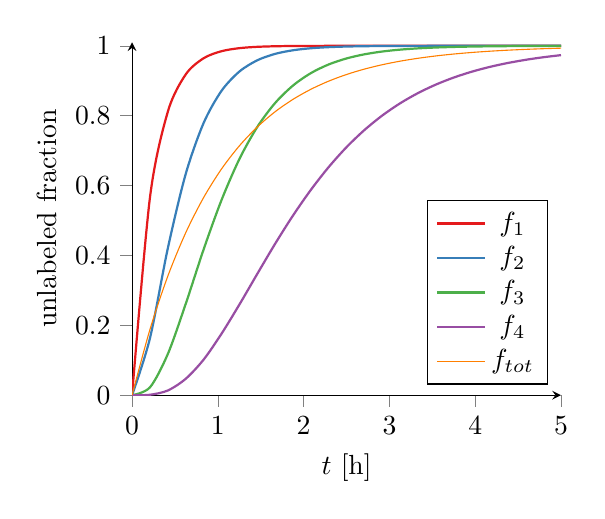
\begin{tikzpicture}
	\begin{axis}[width=200pt,axis x line=bottom, axis y line=left, tick align=outside, domain=0:5, xlabel={$t$ [h]}, ylabel={unlabeled fraction}, ymin=0, ymax=1.01, legend pos=south east]
    	\addplot+[mark=none,smooth,thick] (\x,{ 1 - exp(-4*\x) });
    	\addlegendentry{$f_1$}
    	\addplot+[mark=none,smooth,thick] (\x,{ 1 + 3*exp(-4*\x) - 4*exp(-3*\x) });
    	\addlegendentry{$f_2$}
    	\addplot+[mark=none,smooth,thick] (\x,{ 1 - 3*exp(-4*\x) + 8*exp(-3*\x) - 6*exp(-2*\x) });
    	\addlegendentry{$f_3$}
    	\addplot+[mark=none,smooth,thick] (\x,{ 1 + 1*exp(-4*\x) - 4*exp(-3*\x) + 6*exp(-2*\x) - 4*exp(-\x) });
    	\addlegendentry{$f_4$}
    	\addplot+[mark=none,smooth] (\x,{ 1 - exp(-\x) });
    	\addlegendentry{$f_{tot}$}
    \end{axis}
	\end{tikzpicture}
\end{center}

\subsection{2-step assembly process with unknown pool sizes}
Here, we consider the most simple case of protein complex assembly. We assume that we can measure the labeling of the prey protein before and after forming a complex with the bait, denoted \textit{precursor pool} and \textit{bound pool} with the corresponding pool sizes ($s_1$ and $s_2$). As before, at time $t = 0$, any newly synthesized protein would be labeled. Additionally, we assume no degradation and irreversible binding. The only diluting factor is the growth rate $\mu$.

So, we can use the general solution from equation \ref{eq:dilution}, where $\phi_1 = s_1 / (s_1 + s_2)$ and $\phi_2 = 1$:
\begin{eqnarray}
    f_1 &=& 1 - e^{- \mu t / \phi_1} \\
    f_2 &=& 1 - \left(1 - 1 / \phi_1 \right)^{-1} e^{- \mu t / \phi_1} - \left(1 - \phi_1 \right)^{-1} e^{- \mu t}
\end{eqnarray}
We can now rewrite $f_2$ as a function of $f_1$ and thus get rid of $t$:
\begin{eqnarray}
    f_2 &=& 1 + \frac{\phi_1}{1-\phi_1} (1 - f_1) - \frac{1}{1-\phi_1} (1 - f_1)^{\phi_1}
\end{eqnarray}
which is a function that looks like this:
\begin{center}
	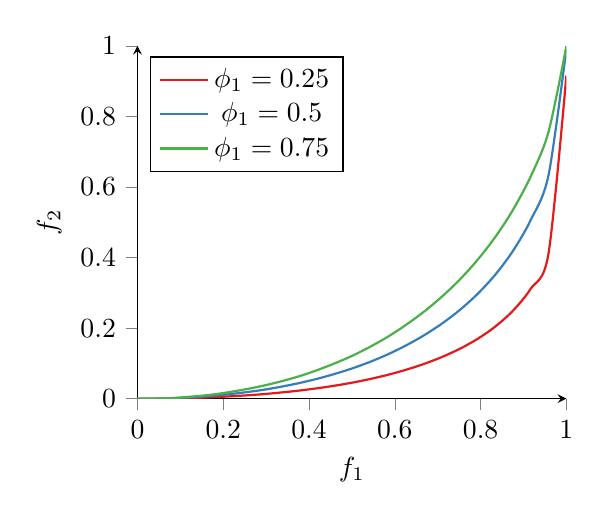
\begin{tikzpicture}[
		declare function={ f2(\x,\y) = 1 + \y/(1-\y)*(1-\x) - 1/(1-\y)*(1-x)^\y ;
		},
	]
	\begin{axis}[width=200pt,axis x line=bottom, axis y line=left, tick align=outside, domain=0:1, xmin=0, xmax=1, xlabel={$f_1$}, ylabel={$f_2$}, ymin=0, ymax=1, legend pos=north west]
    	\addplot+[mark=none,smooth,thick] (\x,{ f2(\x, 0.25) });
    	\addlegendentry{$\phi_1 = 0.25$}
    	\addplot+[mark=none,smooth,thick] (\x,{ f2(\x, 0.5) });
    	\addlegendentry{$\phi_1 = 0.5$}
    	\addplot+[mark=none,smooth,thick] (\x,{ f2(\x, 0.75) });
    	\addlegendentry{$\phi_1 = 0.75$}
	\end{axis}
	\end{tikzpicture}
\end{center}

We can also rewrite the two fraction $f_1$ and $f_2$ as functions of $f_{tot} = 1 - e^{- \mu t}$:
\begin{eqnarray}
    f_1 &=& 1 - (1 - f_{tot})^{1/{\phi_1}} \label{eq:two_step_f1_vs_ftot} \nonumber\\
    f_2 &=& 1 + \frac{\phi_1}{1-\phi_1} (1 - f_{tot})^{1/{\phi_1}} - \frac{1}{1-\phi_1} (1 - f_{tot}) \label{eq:two_step_f2_vs_ftot}
\end{eqnarray}

\begin{center}
	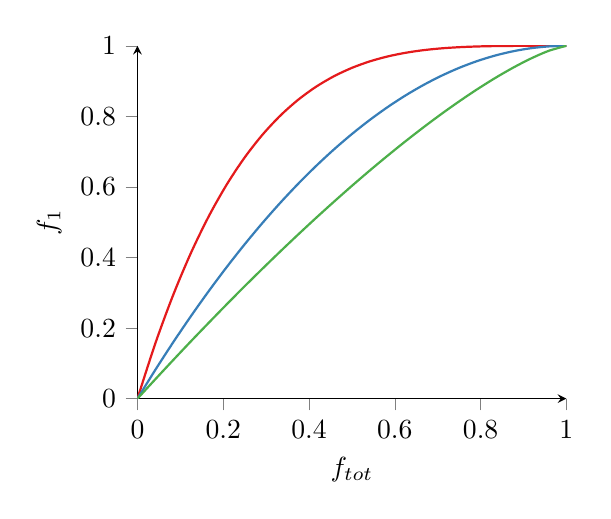
\begin{tikzpicture}[
		declare function={ f1(\x,\y) = 1-(1-\x)^(1/\y) ;
		},
	]
	\begin{axis}[width=200pt,axis x line=bottom, axis y line=left, tick align=outside, domain=0:1, xmin=0, xmax=1, xlabel={$f_{tot}$}, ylabel={$f_1$}, ymin=0, ymax=1, legend pos=south east]
    	\addplot+[mark=none,smooth,thick] (\x,{ f1(\x, 0.25) });
    	\addplot+[mark=none,smooth,thick] (\x,{ f1(\x, 0.5) });
    	\addplot+[mark=none,smooth,thick] (\x,{ f1(\x, 0.75) });
	\end{axis}
	\end{tikzpicture}
	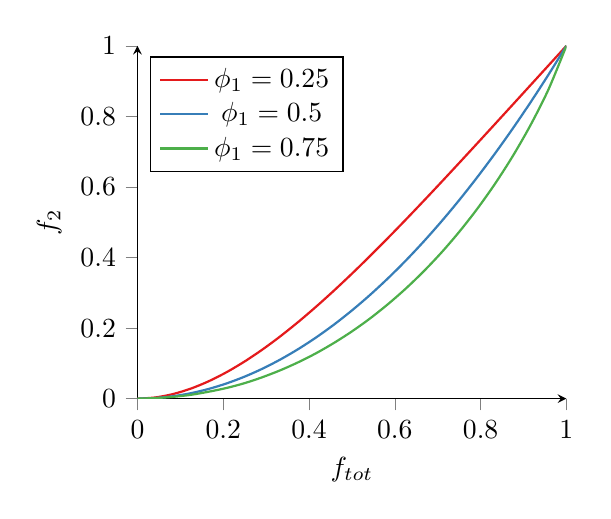
\begin{tikzpicture}[
		declare function={ f2(\x,\y) = 1 + \y/(1-\y)*(1-\x)^(1/\y) - 1/(1-\y)*(1-\x) ;
		},
	]
	\begin{axis}[width=200pt,axis x line=bottom, axis y line=left, tick align=outside, domain=0:1, xmin=0, xmax=1, xlabel={$f_{tot}$}, ylabel={$f_2$}, ymin=0, ymax=1, legend pos=north west]
    	\addplot+[mark=none,smooth,thick] (\x,{ f2(\x, 0.25) });
    	\addlegendentry{$\phi_1 = 0.25$}
    	\addplot+[mark=none,smooth,thick] (\x,{ f2(\x, 0.5) });
    	\addlegendentry{$\phi_1 = 0.5$}
    	\addplot+[mark=none,smooth,thick] (\x,{ f2(\x, 0.75) });
    	\addlegendentry{$\phi_1 = 0.75$}
	\end{axis}
	\end{tikzpicture}
\end{center}

If measuring both $f_1$ and $f_{tot}$ is possible, there is an analytical solution for $\phi_1$:
\begin{eqnarray}
    \phi_1 &=& \frac{\ln(1-f_{tot})}{\ln(1-f_{1})}
\end{eqnarray}
but unfortunately, we can typically only measure $f_2$ and $f_{tot}$, so solving for $\phi_1$ must be done numerically.

\begin{center}
	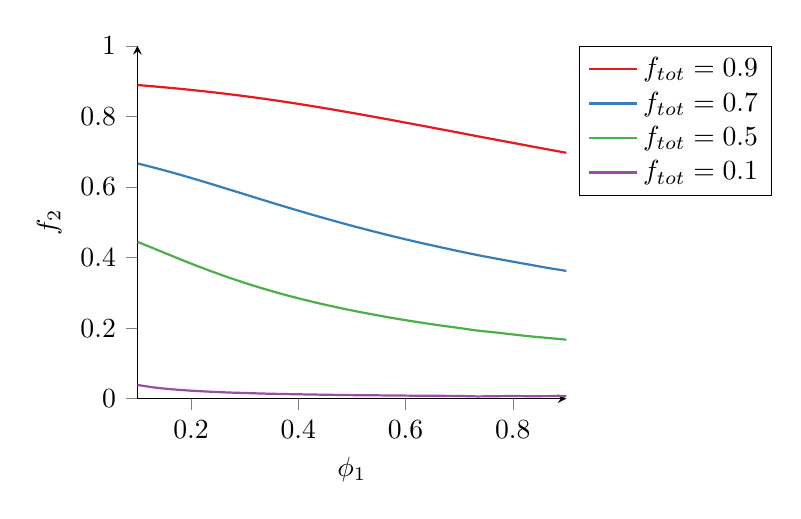
\begin{tikzpicture}[
		declare function={ f2(\x,\y) = 1+\x/(1-\x)*(1-\y)^(1/\x) - 1/(1-\x)*(1-\y);
		},
	]
    \begin{axis}[width=200pt,axis x line=bottom, axis y line=left, tick align=outside, domain=0.1:0.9, xlabel={$\phi_1$}, ylabel={$f_2$}, ymin=0, ymax=1, legend pos=outer north east]
    	\addplot+[mark=none,smooth,thick] (\x,{ f2(\x, 0.9) });
    	\addlegendentry{$f_{tot} = 0.9$}
    	\addplot+[mark=none,smooth,thick] (\x,{ f2(\x, 0.7) });
    	\addlegendentry{$f_{tot} = 0.7$}
    	\addplot+[mark=none,smooth,thick] (\x,{ f2(\x, 0.5) });
    	\addlegendentry{$f_{tot} = 0.5$}
    	\addplot+[mark=none,smooth,thick] (\x,{ f2(\x, 0.1) });
    	\addlegendentry{$f_{tot} = 0.1$}
	\end{axis}
	\end{tikzpicture}
\end{center}


\subsection{3-step assembly process with unknown pool sizes}
Another common case we consider, is similar to the 2-step assembly, except that bound proteins can continue on to an \textit{inaccessible pool} with an unknown size.

So, we can use the general solution from equation \ref{eq:dilution}, where $\phi_1 = s_1 / (s_1 + s_2 + s_3)$, $\phi_2 = s_2 / (s_2 + s_3)$ and $\phi_3 = 1$:
\begin{eqnarray}
    f_1 &=& 1 - e^{- \mu t / \phi_1} \nonumber\\
    f_2 &=& 1 - \left(1 - \phi_2 / \phi_1 \right)^{-1} e^{- \mu t / \phi_1} - \left(1 - \phi_1 / \phi_2 \right)^{-1} e^{- \mu t / \phi_2} \nonumber\\
    f_3 &=& 1 - \left(1 - \phi_2 / \phi_1 \right)^{-1} \left(1 - \phi_3 / \phi_1 \right)^{-1} e^{- \mu t / \phi_1} - \left(1 - \phi_1 / \phi_2 \right)^{-1} \left(1 - \phi_3 / \phi_2 \right)^{-1} e^{- \mu t / \phi_2} - \nonumber\\
    && \left(1 - \phi_1 / \phi_3 \right)^{-1} \left(1 - \phi_2 / \phi_3 \right)^{-1} e^{- \mu t / \phi_3}
\end{eqnarray}

As before, we only care about $f_2$ and $f_{tot}$ since they are measurable, so we express one as a function of the other:
\begin{eqnarray}
    f_{tot} &=& 1 - e^{- \mu t}\nonumber\\
    f_2 &=& 1 + \frac{\phi_1}{\phi_2 - \phi_1} (1 - f_{tot})^{1/{\phi_1}} - \frac{\phi_2}{\phi_2-\phi_1} (1 - f_{tot})^{1/{\phi_2}} \label{eq:three_step_f2}
\end{eqnarray}

Importantly, there is a complete symmetry between $\phi_1$ and $\phi_2$ (i.e. $f_2(\phi_1, \phi_2) = f_2(\phi_2, \phi_1)$, and that means that if we use this function to fit experimental data, we would not be able to distinguish between two equivalent solutions ($\phi_1$, $\phi_2$) and ($\phi_2$, $\phi_1$).

The effect of a large inaccessible pool (small $\phi_2$) is to shift the curves to the left (i.e. make the labeling of $f_2$ occur at earlier and at lower levels of $f_{tot}$), as seen in the following example:
\begin{center}
	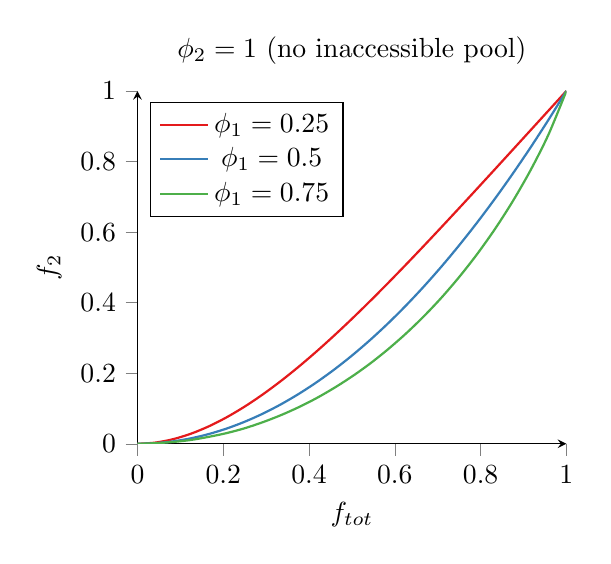
\begin{tikzpicture}[
		declare function={ f2(\x,\y,\z) = 1 + \y/(\z - \y)*(1-\x)^(1/\y) - \z/(\z - \y)*(1-\x)^(1/\z);
		},
	]
	\begin{axis}[title={$\phi_2 = 1$ (no inaccessible pool)}, width=200pt,axis x line=bottom, axis y line=left, tick align=outside, domain=0:1, xlabel={$f_{tot}$}, ylabel={$f_2$}, ymin=0, ymax=1, legend pos=north west]
    	\addplot+[mark=none,smooth,thick] (\x,{ f2(\x, 0.25, 1) });
		\addlegendentry{$\phi_1 = 0.25$}
		\addplot+[mark=none,smooth,thick] (\x,{ f2(\x, 0.5, 1) });
		\addlegendentry{$\phi_1 = 0.5$}
		\addplot+[mark=none,smooth,thick] (\x,{ f2(\x, 0.75, 1) });
		\addlegendentry{$\phi_1 = 0.75$}
	\end{axis}
	\end{tikzpicture}
	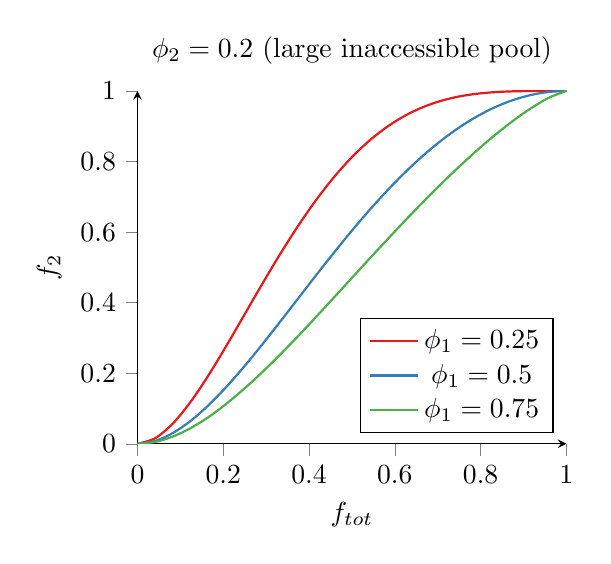
\begin{tikzpicture}[
		declare function={ f2(\x,\y,\z) = 1 + \y/(\z - \y)*(1-\x)^(1/\y) - \z/(\z - \y)*(1-\x)^(1/\z);
		},
	]
	\begin{axis}[title={$\phi_2 = 0.2$ (large inaccessible pool)}, width=200pt,axis x line=bottom, axis y line=left, tick align=outside, domain=0:1, xlabel={$f_{tot}$}, ylabel={$f_2$}, ymin=0, ymax=1, legend pos=south east]
    	\addplot+[mark=none,smooth,thick] (\x,{ f2(\x, 0.25, 0.2) });
		\addlegendentry{$\phi_1 = 0.25$}
    	\addplot+[mark=none,smooth,thick] (\x,{ f2(\x, 0.5, 0.2) });
    	\addlegendentry{$\phi_1 = 0.5$}
    	\addplot+[mark=none,smooth,thick] (\x,{ f2(\x, 0.75, 0.2) });
    	\addlegendentry{$\phi_1 = 0.75$}
	\end{axis}
	\end{tikzpicture}
\end{center}
As expected, the figure on the left ($\phi_2 = 1$) is identical to the one in the previous section (2-step model). We can conclude that $f_2$ decreases with $\phi_1$ as well as $\phi_2$.

\subsection{Solution for the limit of equal \texorpdfstring{$\phi$}{phi} values}
The function in equation \ref{eq:three_step_f2} is not defined for $\phi_1 = \phi_2$ (since we have a 0 divided by 0 situation). However, we can solve the limit using L'H\^{o}pital's rule (we assume $\phi_1$ is constant and derive the numerator and denominator according to $\phi_2$):
\begin{eqnarray}
	f_2 &=& 
	\frac{\phi_2 - \phi_1 + \phi_1 (1-f_{tot})^{1/{\phi_1}} - \phi_2 (1-f_{tot})^{1/{\phi_2}}}{\phi_2 - \phi_1}
	\nonumber\\
	&=& \frac{1 - (1-f_{tot})^{1/{\phi_2}} + \phi_2 \cdot \phi_2^{-2} \cdot \ln{(1-f_{tot})} \cdot(1-f_{tot})^{1/{\phi_2}}}{1}
	\nonumber\\
	&=& 1 - \left(1 - \frac{\ln{(1-f_{tot})}}{\phi_2} \right) \cdot (1-f_{tot})^{1/{\phi_2}}
\end{eqnarray}
where we used the formula $\frac{\partial a^{f(x)}}{\partial x} = \frac{\partial f}{\partial x}\ln(a) a^{f(x)}$. This is what this function looks like for several values of $\phi_1 = \phi_2 = \phi$:
\begin{center}
	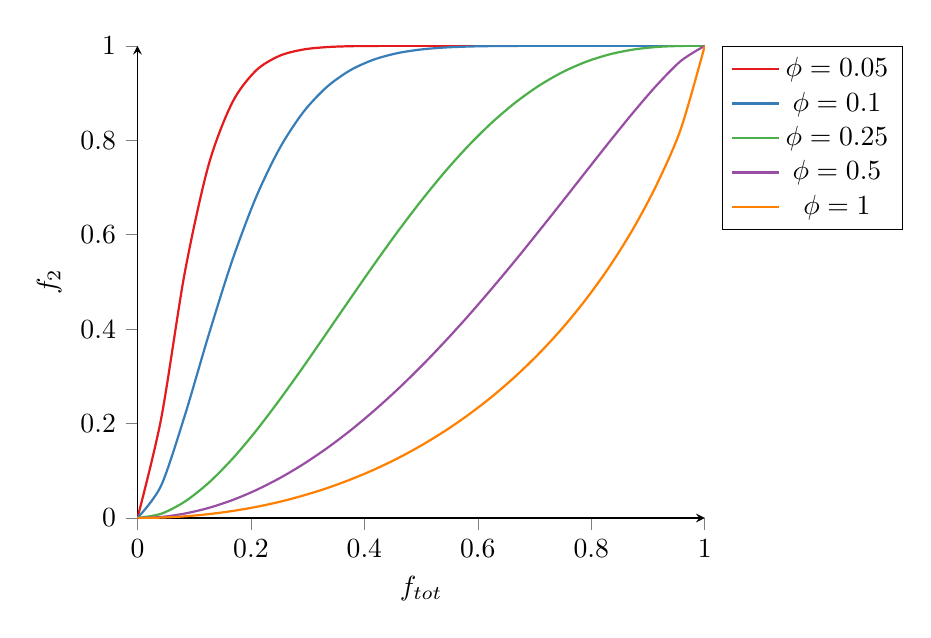
\begin{tikzpicture}[
		declare function={ f2app(\x,\y) = 1 - (1 - ln(1-\x) / \y) * (1-\x) ^ (1/\y);
		},
	]
	\begin{axis}[width=250pt,axis x line=bottom, axis y line=left, tick align=outside, domain=0:1, xmin=0, xmax=1, xlabel={$f_{tot}$}, ylabel={$f_2$}, ymin=0, ymax=1, legend pos=outer north east]
	\addplot+[mark=none,smooth,thick] (\x,{ f2app(\x, 0.05) });
	\addlegendentry{$\phi = 0.05$}
	\addplot+[mark=none,smooth,thick] (\x,{ f2app(\x, 0.1) });
	\addlegendentry{$\phi = 0.1$}
	\addplot+[mark=none,smooth,thick] (\x,{ f2app(\x, 0.3) });
	\addlegendentry{$\phi = 0.25$}
	\addplot+[mark=none,smooth,thick] (\x,{ f2app(\x, 0.6) });
	\addlegendentry{$\phi = 0.5$}
	\addplot+[mark=none,smooth,thick] (\x,{ f2app(\x, 1) });
	\addlegendentry{$\phi = 1$}
	\end{axis}
	\end{tikzpicture}
\end{center}

\subsection{Observability of \texorpdfstring{$\phi_1$}{phi1} and \texorpdfstring{$\phi_2$}{phi2}}
It is noteworthy, that even though $f_2$ has two degrees of freedom ($\phi_1$ and $\phi_2$), the function is \textit{almost} redundant in parameter space, meaning that the shape of $f_2$ is almost constant if $\phi_1 \cdot \phi_2 =$ const. Below is an example for a range of values, where $\phi_1 \cdot \phi_2 = 0.36$. We also compare that to the limit $\phi_1 = \phi_2 = 0.6$.

\begin{center}
	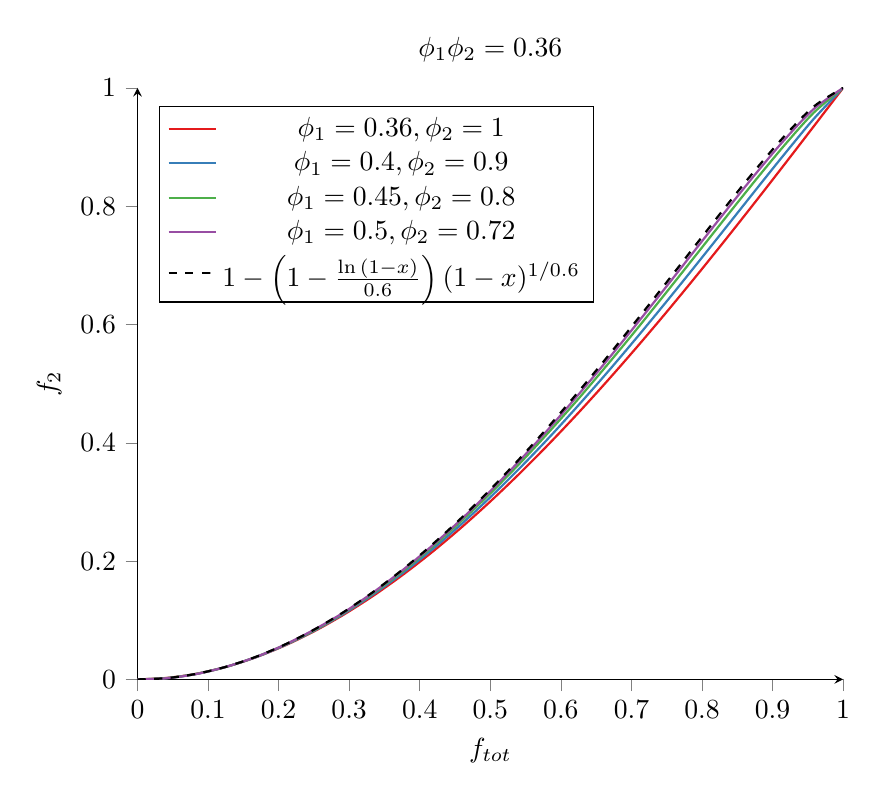
\begin{tikzpicture}[
	declare function={ f2(\x,\y,\z) = 1 + \y/(\z - \y)*(1-\x)^(1/\y) - \z/(\z - \y)*(1-\x)^(1/\z);
	},
	declare function={ f2app(\x,\y) = 1 - (1 - ln(1-\x) / \y) * (1-\x) ^ (1/\y);
	},
	]
	\begin{axis}[title={$\phi_1 \phi_2 = 0.36$}, width=300pt,axis x line=bottom, axis y line=left, tick align=outside, domain=0:1, xlabel={$f_{tot}$}, ylabel={$f_2$}, ymin=0, ymax=1, legend pos=north west]
		\addplot+[mark=none,smooth,thick] (\x,{ f2(\x, 0.36, 1) });
		\addlegendentry{$\phi_1 = 0.36, \phi_2 = 1$}
		\addplot+[mark=none,smooth,thick] (\x,{ f2(\x, 0.4, 0.9) });
		\addlegendentry{$\phi_1 = 0.4, \phi_2 = 0.9$}
		\addplot+[mark=none,smooth,thick] (\x,{ f2(\x, 0.45, 0.8) });
		\addlegendentry{$\phi_1 = 0.45, \phi_2 = 0.8$}
		\addplot+[mark=none,smooth,thick] (\x,{ f2(\x, 0.5, 0.72) });
		\addlegendentry{$\phi_1 = 0.5, \phi_2 = 0.72$}
		\addplot+[color=black,dashed,mark=none,smooth,thick] (\x,{ f2app(\x, 0.6) });
		\addlegendentry{$1 - \left(1 - \frac{\ln{(1 - x)}}{0.6} \right) (1 - x)^{1/{0.6} }$}
	\end{axis}
	\end{tikzpicture}
\end{center}

This means, that if we try to fit these parameters to measured data, we might not be able to distinguish between a set of nearly equivalent solutions (with the same $\phi_1 \cdot \phi_2$ value).

\subsubsection{Example with pool size as parameters}
Given two scenarios, where the pool size ratios are 4:3:3 and 5:2:3, the $f_2$ trajectory will look exactly the same.

\begin{center}
	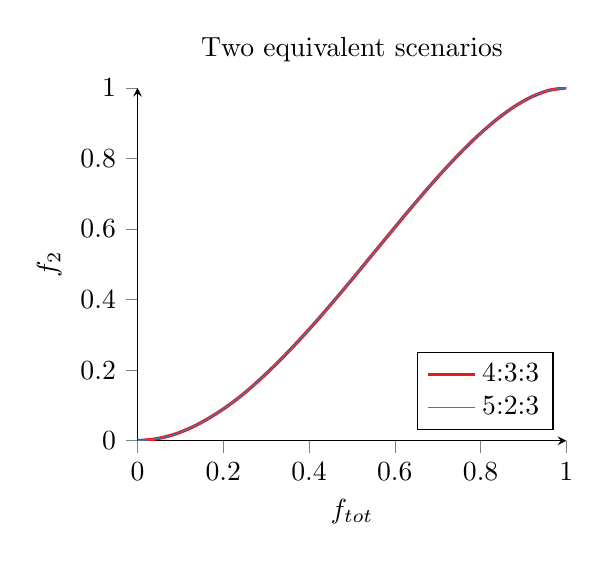
\begin{tikzpicture}[
	declare function={ f2(\x,\y,\z) = 1 + \y/(\z - \y)*(1-\x)^(1/\y) - \z/(\z - \y)*(1-\x)^(1/\z);
	},
	]
	\begin{axis}[title={Two equivalent scenarios}, width=200pt,axis x line=bottom, axis y line=left, tick align=outside, domain=0:1, xlabel={$f_{tot}$}, ylabel={$f_2$}, ymin=0, ymax=1, legend pos=south east]
	\addplot+[mark=none,smooth,very thick] (\x,{ f2(\x, 0.4, 0.5) });
	\addlegendentry{4:3:3}
	\addplot+[mark=none,smooth] (\x,{ f2(\x, 0.5, 0.4) });
	\addlegendentry{5:2:3}
	\end{axis}
	\end{tikzpicture}
\end{center}

\section{Linear reversible pathway with dilution}
In this section, we relax our assumption that all reactions are irreversible, but keep focusing on linear pathways whose fluxes are determined by dilution. Unfortunately, the solution for general pathway lengths is extremely complex. Therefore, the only analytical solution we will discuss here is the case of $n = 2$.

\subsection{2-step assembly with reversibility}

\begin{equation}
    \rightarrow S_0 
    \rightarrow \underset{\downarrow}{S_1}
    \rightleftarrows \underset{\downarrow}{S_2}
\end{equation}
As usual, we assume that the system is at balanced growth, so that the dilution fluxes are proportional to their pool sizes, i.e. $\mu s_i$. So:
\begin{eqnarray}
    v_{1 \rightarrow 2} &=& \mu s_2 + v_{2 \rightarrow 1}\\
    v_{0 \rightarrow 1} &=& \mu (s_1 + s_2)
\end{eqnarray}

For simplicity, we define $x \equiv v_{2 \rightarrow 1} / (\mu s_2)$, therefore:
\[\mathbf{V} =
    \begin{bmatrix}
        0 & \mu (s_1 + s_2) & 0\\
        0 & 0 & \mu s_2 (1 + x) \\
        0 & \mu s_2 x & 0 \\
        0 & 0 & 0 \\
    \end{bmatrix}
\]

The we use the formula $\mathbf{M} = \text{diag}(\vec{s})^{-1} \cdot \left( \mathbf{V}^\top - \text{diag}(\mathbf{V}^\top~\vec{1}_n) \right)$ to get

\[
\mathbf{M} = \mu \cdot 
    \begin{bmatrix}
        0 & 0 & 0  \\
        1 + s_2/s_1 & - 1 - (1+x) s_2 / s_1 & x s_2 / s_1 \\
        0 & 1+x  & -1-x
    \end{bmatrix}
\]
As before, we can reduce the number of parameters by setting $\phi_1 \equiv \frac{s_1}{s_1+s_2}$:
\[
\mathbf{M} = \mu \cdot 
    \begin{bmatrix}
        0 & 0 & 0  \\
        1/\phi_1 & - 1 - (1+x)(1/\phi_1-1) & x (1/\phi_1-1) \\
        0 & 1+x  & -1-x
    \end{bmatrix}
\]
and then find the Jordan normal form for $\mathbf{M}$ using \href{https://www.sympy.org/}{Sympy} while solving for $\mathbf{P}~\text{diag}\left(\mathbf{P}^{-1} ~\finit\right)$:
\begin{eqnarray}
\mathbf{J} = \mu \cdot
  \begin{bmatrix}
    0 & 0 & 0 \\
    0 & -\frac{x+1}{\phi_1} & 0 \\
    0 & 0 & -1
\end{bmatrix}
~~~~
\mathbf{P}~\text{diag}\left(\mathbf{P}^{-1} ~\finit\right) =
    \begin{bmatrix}
        1 & 0 & 0 \\
        1 & \frac{\phi_1 - 1}{x + 1 - \phi_1} & -\frac{x}{x + 1 - \phi_1} \\
        1 & \frac{\phi_1}{x + 1 - \phi_1} & -\frac{x+1}{x + 1 - \phi_1} 
    \end{bmatrix}
\end{eqnarray}
We can continue to simplify this expression by defining $\phi_1' \equiv \phi_1/(1+x)$ and get the following:
\begin{eqnarray}
    f(t) = \mathbf{P}~\text{diag}\left(\mathbf{P}^{-1} ~\finit\right) \cdot e^{\mathbf{J}t} = 
    \begin{bmatrix}
        1 & 0 & 0 \\
        1 & \frac{\bar{\phi}_1 - 1/(1+x)}{1 - \phi_1'} & -\frac{x/(1+x)}{1 - \phi_1'} \\
        1 & \frac{\phi_1'}{1 - \phi_1'} & -\frac{1}{1 - \phi_1'}
    \end{bmatrix} \cdot 
    \begin{bmatrix}
        1 \\
        e^{-\mu\,t / \phi_1'} \\
        e^{-\mu\,t}
    \end{bmatrix}
\end{eqnarray}

And focusing only on $f_2(t)$ we get this final expression
\begin{eqnarray}
    f_2 ~=~ 1 + \frac{\phi_1'}{1 - \phi_1'} (1-f_{tot})^{1/\phi_1'} ~-~ \frac{1}{1 - \phi_1'} (1-f_{tot})
\end{eqnarray}
where again we substituted $e^{\mu\,t}$ with $1-f_{tot}$.

This equation is completely identical to the solution for $f_2$ in the 2-step irreversible model (Equation \ref{eq:two_step_f2_vs_ftot}), where $\phi_1'$ replaces $\phi_1$. That means that for any $x > 0$, we will be able to fit $f_2$ as a function of $f_{tot}$ precisely also with an irreversible model, and the precursor pool $\phi_1$ will be underestimated by a factor of $1+x$.

\subsection{Analytical solution for maturation time}
We define the maturation time $t_{1/2}$ as the time after which a protein that starts in $S_1$ to have a 50\% chance of reaching $S_2$. 

In the 2-step reversible model, the total flux from $S_1$ to $S_2$ is $\mu s_2 (1+x)$, and therefore the chance of any molecule in $S_1$ to make the transition in a short time interval $dt$ is $\mu s_2/s_1 (1+x) dt$. We can replace $s_2/s_1$ with $1/\phi_1 - 1$.

We denote by $P(t)$, the probability that our protein of interest has moved to $S_2$ (matured) before time $t$. The chance of making the transition exactly between $t$ and $t+dt$ is the probability it did not happen already before $t$ (which is $1 - P(t)$) times the probability we just calculated earlier:
\begin{eqnarray}
    dP &=& P(t + dt) - P(t) = \left(1 - P(t)\right) \mu s_2/s_1 (1+x) dt \\
    \int_0^T \frac{1}{1-P} dP &=& \int_0^T s_2/s_1 \mu (1+x)~dt  \\
    -\ln(1-P) &=& s_2/s_1 \mu (1+x)t = (1/\phi_1 - 1)\mu (1+x)t  \\
    t &=& \frac{-\ln(1-P(t))}{\mu (1+x)} \frac{\phi_1}{1 - \phi_1}\,.
\end{eqnarray}

Now, imagine that we fit the precursor pools using data while assuming that the reactions are irreversible. In this case, we are going to underestimate $\phi_1$ by a factor of $(1+x)$, when trying to estimate $t$. To understand how this assumption affects the result, we define our new estimate as:
\begin{eqnarray}
    t' &\equiv& \frac{-\ln(1-P)}{\mu} \cdot \frac{\phi'_1}{1 - \phi'_1} 
    = \frac{-\ln(1-P)}{\mu} \cdot \frac{\phi_1/(1+x)}{1 - \phi_1/(1+x)} \nonumber\\
    &=& \frac{-\ln(1-P)}{\mu (1+x)} \cdot \frac{\phi_1}{1 - \phi_1/(1+x)} 
    = t \cdot \frac{1 - \phi_1}{1 - \phi_1/(1+x)}
\end{eqnarray}
and therefore
\begin{eqnarray}
    1 ~\geq~ \frac{t'}{t} ~>~ 1-\phi_1
\end{eqnarray}
or in other words, if we use an irreversible model to find the maturation, we might underestimate it, but not by more than a factor of $1-\phi_1$.

\clearpage
\section{Fitting measured data}

\subsection{Using the 2-step model}
The common scenario would be that $\tau_i$ are unknown, and we have several time point measurements of some or all $f_i$. In this example, we assume again a 3-step chain, where we measure $f_{tot}$ and $f_2$, and the free parameters are $\phi_1$ and $\phi_2$. 

\subsection{How to infer fluxes from labeling data}

We assume that the data was generated from a system such as in equation \ref{eq:homogenous}, with a diagonalizable matrix $\mathbf{M}$. Then, we can fit our data (which is $\vec{f}$ measured at multiple time points) using the formula $\vec{f}(t) = \mathbf{A} e^{\vec{\lambda} t}$. Then, from equation \ref{eq:homogenous_solution} we know that $\mathbf{P} = \mathbf{A} \mathbf{D}^{-1}$, where $\mathbf{D}$ is some fully ranked diagonal matrix. Even though $\mathbf{D}$ is somehow dependent on $\mathbf{P}$ and $\mathbf{A}$, it wouldn't matter for finding $\mathbf{M}$, since:
\begin{eqnarray}
    \mathbf{M} = \mathbf{P}~\text{diag}(\vec{\lambda})~\mathbf{P}^{-1} = \mathbf{A}\mathbf{D}^{-1}~\text{diag}(\vec{\lambda})~\mathbf{D}\mathbf{A}^{-1} = 
    \mathbf{A}\mathbf{D}^{-1}\mathbf{D}~\text{diag}(\vec{\lambda})~\mathbf{A}^{-1} = 
    \mathbf{A}~\text{diag}(\vec{\lambda})~\mathbf{A}^{-1}
\end{eqnarray}
where $\text{diag}(\vec{\lambda})~\mathbf{D} = \mathbf{D}~\text{diag}(\vec{\lambda})$ since they are both diagonal matrices. Therefore, we can simply ignore the $\mathbf{D}$ matrix altogether, and use the solution:
\begin{eqnarray}
    \mathbf{\bar{V}} = \mathbf{M}^\top~\text{diag}(\vec{s}) = \left(\mathbf{A}~\text{diag}(\vec{\lambda})~\mathbf{A}^{-1} \right)^\top~\text{diag}(\vec{s})
\end{eqnarray}
where $\mathbf{\bar{V}} = \mathbf{V} - \text{diag}(\vec{1}_n~\mathbf{V})$, i.e. the fluxes would be the off-diagonal values of $\mathbf{\bar{V}}$.

\end{document}